\documentclass[10pt]{article}
\usepackage[a4paper, left=1.5cm, right=1.5cm, top=3.5cm]{geometry}
\usepackage[ngerman]{babel}
\usepackage[]{graphicx}
\usepackage{enumitem}
\usepackage{multicol}
\usepackage{amssymb}
\usepackage{breqn}
\usepackage{titlesec}
\usepackage{wrapfig}
\usepackage{blindtext}
\usepackage{lipsum}
\usepackage{caption}
\usepackage{listings}
\usepackage{fancyhdr}
\usepackage{nopageno}
\usepackage{authblk}
\usepackage{amsmath} % tons of math stuff
\usepackage{mathtools} % e.g. alignment within matrix
\usepackage{bm} % provides shorthand for bold in math mode
%\usepackage{esdiff} % provides derivative commands
\usepackage[ISO]{diffcoeff}
\usepackage{xcolor}
\usepackage{csquotes} % e.g. provides \enquote
\fancyhf[]{}

% own fig. env. for multicols
\newenvironment{Figure}
  {\par\medskip\noindent\minipage{\linewidth}}
  {\endminipage\par\medskip}

\begin{titlepage}
    \title{Elektronik Praktikum -- Versuch 0: Einführung und Vorversuch}
    \author[1]{Angelo V. Brade\thanks{s72abrad@uni-bonn.de}}
    \affil[1]{Rheinische Friedrich-Wilhelms-Universität Bonn}
    \date{\today}
\end{titlepage}

\begin{document}
\pagenumbering{gobble}
\maketitle
\newpage

\tableofcontents
\newpage

\pagenumbering{arabic}

\pagestyle{fancy}
\fancyhead[R]{\thepage}
\fancyhead[L]{\leftmark}


\begin{multicols}{2}
	\section{\large Einführung}
	In diesem Versuch werden die folgend zu benutzenden Geräte, Netzgerät für die Versorgungsspannungen, Signalquellen und Messgeräte, wie Oszillographen, betrachtet und verstanden.
	\section{\large Theorie}
	\subsection{Das Netzgerät}
	Das Netzgerät ist eine Eigenentwicklung mit 4 verschiedenen Spannungen:
	\begin{enumerate}[itemsep=0.01mm]
		\item +5 V, ca. 1 A, grüne Steckbuchse
		\item +15 V, ca. 100 mA strombegrenzt, rote Steckbuchse
		\item -15V, ca. 100 mA strombegrenzt, gelbe Steckbuchse
		\item 0 bis 15 V regelbar, ca. 100 mA
	\end{enumerate}
	Die Apperatur ist in Abb. \ref{fig:1.1} dargestellt.
	\begin{Figure}
		\centering
		\includegraphics[width=0.9\linewidth]{Netzgerät.png}
		\captionof{figure}{Netzgerät}
		\label{fig:1.1}
	\end{Figure}
	\subsection{Signalquellen}
	Signalen lassen sich folgende beschreibene Größen zuordnen:\\
	Spitze-Spitze: Die Differenzspannung \(U_{\text{SS}}\), die von der unteren zur oberen Spitze geht.\\
	Spitzenwert: Die Differenzspannung \(U_{\text{S}}\), die von der x-Achse zur oberen Spitze geht.\\
	Effektivwert: Die Spannung \(U_{\text{eff}}=\sqrt{\langle U^2(t)}\rangle\) bei Wechselstrom, die die gleiche Leistung für Gleichstrom hätte.
	Nun lassen sich mit einem Funktionsgenerator verschieden Verläufe, wie Segezahn- oder Sinuskurven mit verschiedenen Frequenzen und Amplituden darstellen.
	\subsection{Messgeräte}
	Die Messgeräte werden unterschieden in Digital- und Analogmessgeräte. Letzteres ist z.B. das Drehspulmessgerät, auch Galvanometer genannt, welches auch schon in zuvoriegen Praktika untersucht wurde. Generell lässt sich meist ein Messgerät in Messverstärker, Bereichswahlnetzwerk und Messwandler unterteilen. Der angelegte Strom durchläuft die Unterteilungen auch in dieser Reihenfolge. Als Digitalmessgerät lässt sich anstatt des Drehspulmessgeräts ein Digitalmultimeter verwenden, welches zusätzlich die Funktionalität auf die Strom- und Widerspannungsmessung erweitert. Neben dem weist dieses einen kleineren Fehler auf.

	Das Oszilloskop lässt sich digital, also auch analog bauen. Für die analoge Variante ist die Elektronenstrahlröre essentiell. Dort wird, ähnlich zu einem Kathodenstrahlröhrenbildschirm, mit einer Kathode Elektronen freigesetzt und dann mit einer Anode beschleunigt. Sie werden erst mit einer zylinderförmigen Elektrode in einem Strahl gebündelt, bevor Sie von Kondensatoren in eine x- und y-Richtung abgelengt werden. Die Apperatur ist in Abb. \ref{fig:1.2} skizziert.

	\begin{Figure}
		\centering
		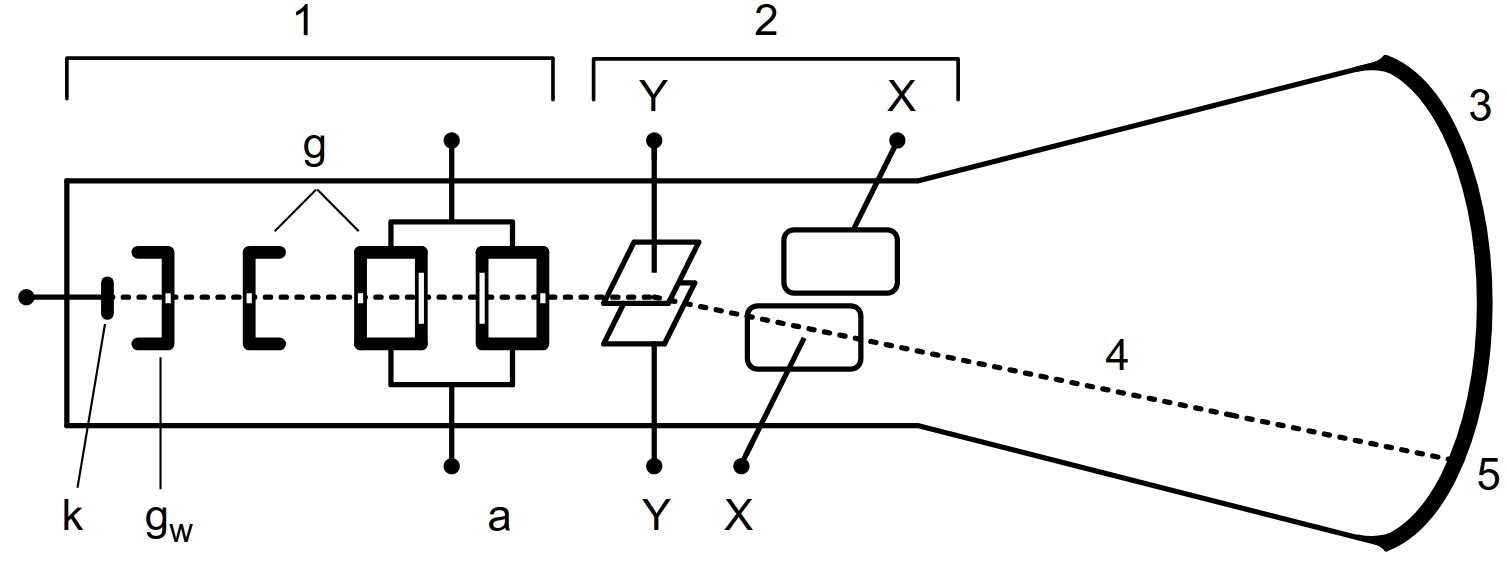
\includegraphics[width=0.9\linewidth]{Osziloskop.png}
		\captionof{figure}{Straherzeugung und Ablenkung der Elektronenstrahlröhre}
		\label{fig:1.2}
	\end{Figure}

	Die Spannungen des Kondesators der y-Richtung wird durch das zu messende Signal geliefert. Die Spannung des Kondesators der x-Richtung wird hingegen intern konstant vergrößert und bei erreichen der Schirmbreite zurückgesetzt. Um zwei Signale zu erzeugen, wird zwischen beiden eingehenden Spannung mit 500 kHz alterniert. Durch Floureszenz und Trägheit des Auges erscheinen dann beide Signale gleichzeitig auf dem Schirm.

	Gelegentlich ist eine Synchronisation des Signals mithilfe eines Triggers erforderlich. Dazu wird ein Sägezahnsignal als sog. Trigger Impuls angelegt.

	Um einen Phasenvergleich durchzuführen lassen sich mit dem XY-Betrieb z.B. Lissajous-Figuren darstellen. Dafür werden die anliegenden Signal jeweils auf eine Achse gelegt.
	\subsection{Anstiegszeit}
	Aufgrund von Impedanzen in dem Funktionsgenerators und Oszilloskops, sowie der Frequenzbandbreite eines Geräts, haben Singal eine endliche Anstiegzeit in ihrer Spannung. Allgemein lässt sich jedes Gerät in 1. Ordnung durch einen Tiefpass beschreiben. Dies lässt sich anschaulich an einem Koaxialkabel verstehen, wobei der Innere und Äußere Lieter einen Kondensator bilden und, wie bei dem Herz'schen Dipol, das Kabel insgesammt eine Spule mit null Windungen darstellen. So lässt sich über die Grenzfrequenz dieses vereinfachten RC-Tiefpasses eine Bandbreite \[B=f_{\text{grenz}}=\frac{1}{2\pi RC}=\frac{1}{2\pi \tau}\] definieren. Dabei führen wir die Zeitkonstante \(\tau=RC\) ein, die außerhalb dieses Rahmens noch weitere Bedeutungen mit sich trägt.

	Oft wird die Anstiegszeit \(\Delta t\) angegeben, die die Zeitdifferenz von 10\% zu 90\% der Amplitude des Signals ist. Ferner wird noch gezeigt, dass \(B\cdot\Delta t \approx 0.35\).
	\section{\large Voraufgaben}

	\subsection{Aufgabe A}
	Für eine Spannung \(U(t)=U_0\sin{\omega t}\) ist \(U_{\text{SS}}=2 \cdot U0\), \(U_{\text{S}}=U_0\) und \(U_{\text{eff}}=\frac{1}{\sqrt{2}}U_0\). Letzteres wurde wegen der Definition von \(U_{\text{eff}}=\sqrt{\langle U^2(t)}\rangle\) mit der trivialen Sinusintegration von 0 bis \(f^{-1}\) durgeführt.

	\subsection{Aufgabe B}
	Für eine Spannung von \(U_S=10\) V ist \(U_{\text{eff}} = 10\) V, da durch die quadrierung die Integration sich zu \(\frac{U_S^2}{f}\) ergibt.
	\subsection{Aufgabe C}
	\[U_n                                 & =U_0 \frac{R_n}{R_n+R_i}\]
	Wähle \(U_n\in \{U_1,U_2\}\) und setzt über \(U_0\) gleich.
	\begin{align*}
		\Rightarrow U_1 \frac{R_1+R_i}{R_1}                & =U_2 \frac{R_2+R_i}{R_2}                \\
		\Rightarrow U_1 \left(1+\frac{R_i I_1}{U_1}\right) & =U_2 \left(1+\frac{R_i I_2}{U_2}\right) \\
		\Rightarrow U_1 + R_i I_1                          & = U_2 + R_I I_2                         \\
		\Rightarrow R_i(I_1 - I_2)                         & = U_2 - U_1                             \\
		\Rightarrow R_i                                    & = \frac{U_2 - U_1}{I_1 - I_2}
	\end{align*}
	Mit \(U_2 = 20\text{ V}_{\text{SS}}\), \(R_2= \infty \Rightarrow I_2=0 \text{ A}_{\text{SS}}\) und \(U_1 = 10\text{ V}_{\text{SS}}\), \(R_1=50 \text{ }\Omega \Rightarrow I_1=0.2 \text{ A}_{\text{SS}}\) folgt \(R_i = 50 \text{ }\Omega\).
	\subsection{Aufgabe D}
	Um sich das Oszilloskop vertrauter zu machen betrachten und vergleichen wir Abb. \ref{fig:1.3} mit Abb. \ref{fig:1.4}.
	\begin{Figure}
		\centering
		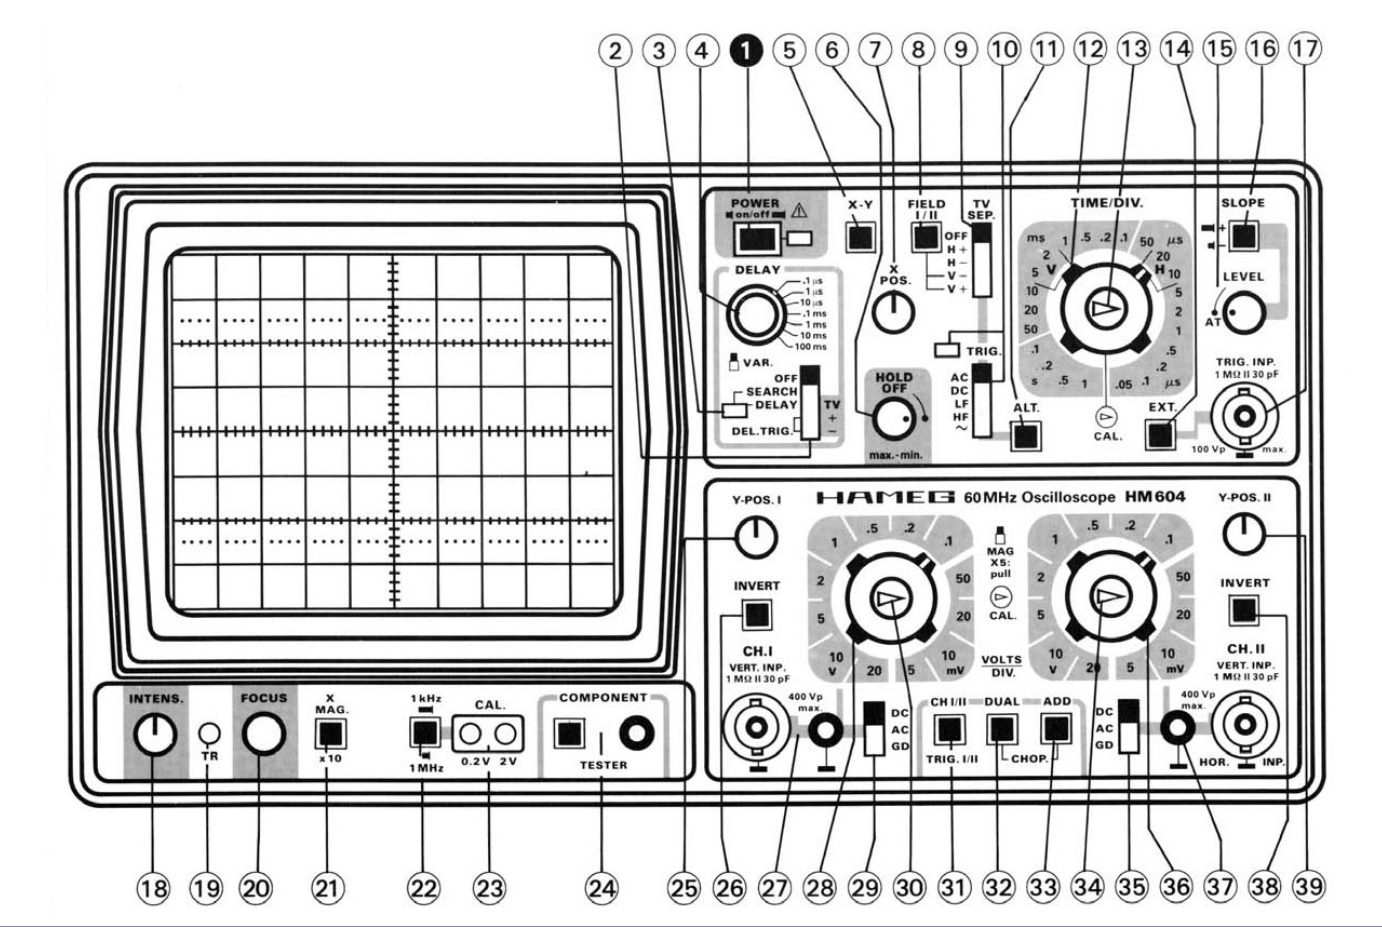
\includegraphics[width=0.9\linewidth]{OszI_font.png}
		\captionof{figure}{Frontalansicht des Oszilloskopen}
		\label{fig:1.3}
	\end{Figure}
	\begin{Figure}
		\centering
		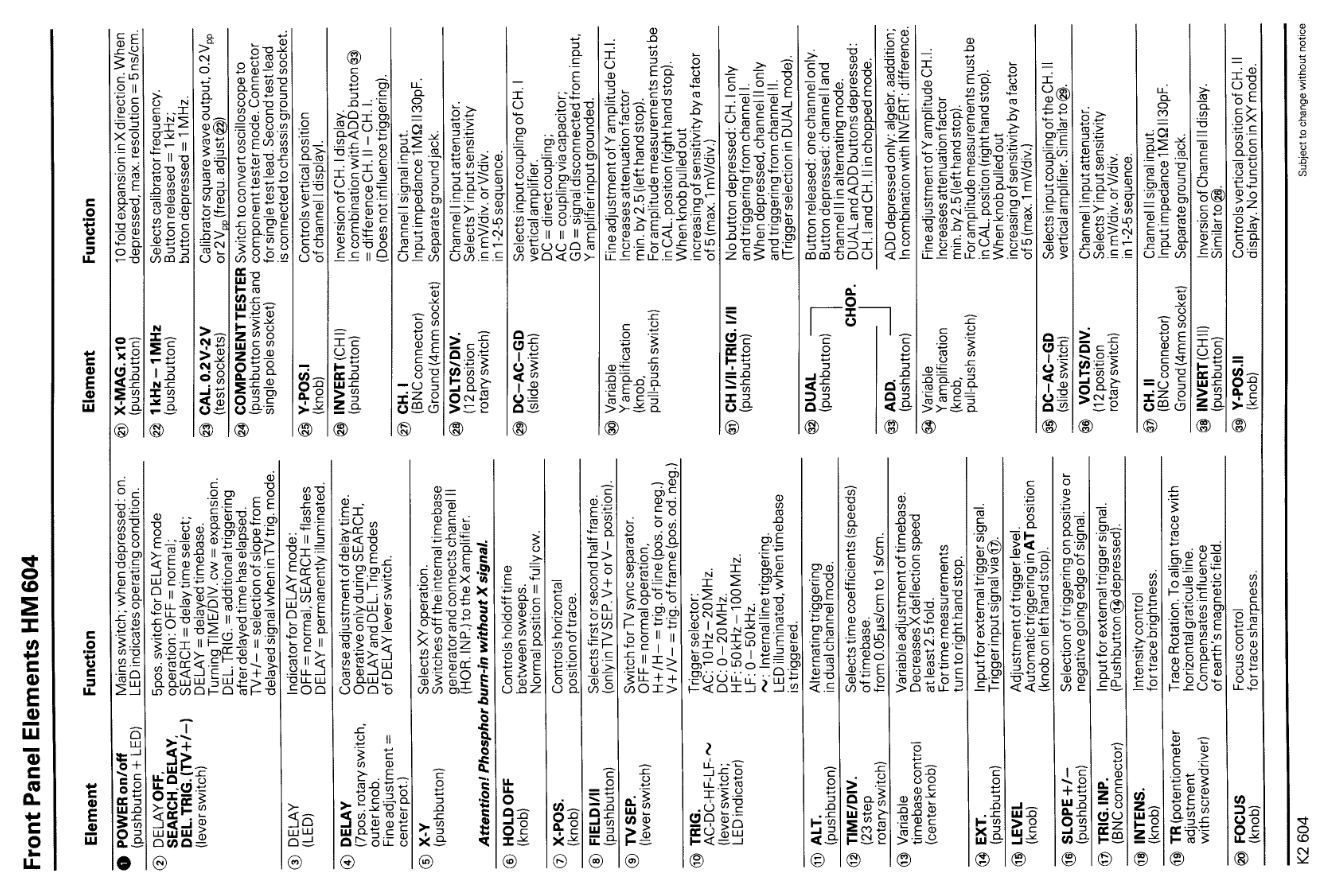
\includegraphics[angle=270, origin=c,width=0.9\linewidth]{oszi_manuel.png}
		\captionof{figure}{Beschriftung des Oszilloskopen}
		\label{fig:1.4}
	\end{Figure}
	\subsection{Aufgabe E}
	Um zu Zeigen, dass \(\Delta t \cdot B \approx 0.35\), müssen wir mit \[U(t)=U_0 \left[1 - \exp{(-\frac{t}{\tau})}\right]\] die Zeitpunkte \(t_1\) und \(t_2\) berechnen.
	\begin{align}
		U(t)          & = U_0\left[1-\exp{(-\frac{t}{\tau})}\right]\\
		\Rightarrow t & =-\tau\ln{\left(1-\frac{U(t)}{U_0}\right)}
	\end{align}
Mit \(U(t_1)=0.1U_0\) und \(U(t_2) = 0.9U_0\) ergibt sich
\begin{align}
  \Delta t &= t_2 - t_1 \\
           &= \tau\ln{0.9} - \tau\ln{0.1}\\
           &= \tau\ln{9}
\end{align}
Somit erhalten wir
\begin{align}
  B\cdot\Delta t &= \frac{1}{2\pi\tau} \cdot \Delta t\\
  &= \frac{1}{2\pi\tau}\tau\ln{9}\approx 0.35
\end{align}

\end{multicols}

\end{document}
